\section{Grading of Categories}

\begin{comment}
The structure of Wikipedia could be considered confusing since anyone can edit. This means that the underlying category structure of Wikipedia contains lots of links between all categories. 

This means that it is possible to reach almost all articles from each category. 

This means that there are categories that reach lots of other categories. These should not be considered as important as the other categories. A program was made to find these categories. 

There are 28 top categories (direct subcategories of %\emph{Main Topic Classifications}). 

The main assumption is that if a category leads to many of the top categories, it is possible to reach lots of articles which are not associated with the category. 

%\begin{code}
Eksempel på hvordan kategorier finner artikler som ikke har noen sammenheng med kategorien.
%\end{code}

If a category leads to many of these 
The top categories (28) leads to lots of subcategories. 

% Fan
Another way of finding categories that does not provide information about the path, is to find all categories with many parent categories and with many subcategories since this means that they easily can reach categories not relevant for the category. 

Hence a program was made to find the number of parent categories and subcategories for each category. 
\end{comment}

Many articles can be reached from categories that are not describing of the content at all, for instance is the article about \emph{Ole-Johan Dahl} (the Norwegian programmer) found from links from the category \emph{people}, but also found from links from the categories \emph{politics} and \emph{arts} (see Figure \ref{fig:olejohandahl_paths}). When all paths are found for all Wikipedia articles, the next step was to grade each path depending on how well they describe the article. 

%grade the paths to find the paths most helpful for describing the article's content. 

\begin{figure}[h]
\centering
\begin{lstlisting}
ole-johan dahl:
*people/people categories by parameter/categories by nationality/academics by nationality/norwegian academics/faculty by university or college in norway/university of oslo faculty

[...]

*politics/political activism/leadership/management/quality/software quality/formal methods/formal methods people

[...]

*arts/aesthetics/design/software design/data modeling/formal methods/formal methods people

\end{lstlisting}
\caption[Example of variety in article paths]{Some of the paths for the article about \emph{Ole-Johan Dahl}.}
\label{fig:olejohandahl_paths}
\end{figure}

\subsection{Grading based on Inlinks and Outlinks} % eller: Grading based on inlink and outlinks 
\subsubsection{Inlinks and Outlinks of Categories}
Each category in Wikipedia has a set of parent categories i.e., categories that lead to the current category, and a set of subcategories i.e., categories that can be reached from the current category. The size of these sets for a given category can be notated as 
\begin{itemize}
\item \emph{Inlink} = number of parent categories
\item \emph{Outlink} = number of subcategories
\end{itemize}
Figure \ref{fig:Categorywparentandsub} is a demonstration of how  \emph{inlink} and \emph{outlink} are connected to a category, and gives the idea that a catgory with high \emph{inlink} and \emph{outlink} are more likely to be visited when looking for paths for an article. 
\begin{figure}[h]
\centering
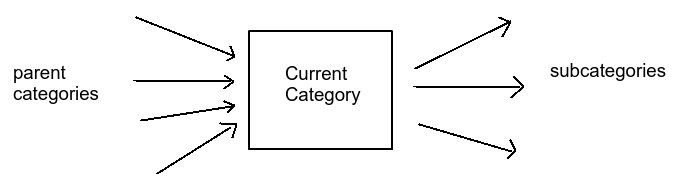
\includegraphics[width=\textwidth]{Chapters/Implementation/Grading/category_parent_sub}
\caption[Example of \emph{inlink} and \emph{outlink} for a category]{Example of how a category has links from parent categories and links to its subcategories. \emph{inlink} for the category is 4 and \emph{outlink} for the category is 3.}
\label{fig:Categorywparentandsub}
\end{figure}


The first assumption is that categories with high \emph{inlink} can be reached from categories that are not about the same. 

%great rift valley: 5, 31
\begin{figure}[h]
\centering
\begin{lstlisting}
INSERT EXAMPLE HERE: 
\end{lstlisting}
\caption{Caption}
\label{fig:my_label}
\end{figure}


\begin{figure}[h]
\centering
\begin{lstlisting}
ole-johan dahl:
*politics/political activism/leadership/management/quality/software quality/formal methods/formal methods people
\end{lstlisting}
\caption{Example of how \emph{politics} can reach the article about \emph{Ole-Johan Dahl}}
\label{fig:politicstosoftware}
\end{figure}
%quality: 9, 3
%management: 31, 5
The next assumption is that categories with a high number for \emph{outlink} are more likely to reach categories not relevant since they can reach far in all the subcategories' directions. Figure \ref{fig:politicstosoftware} shows how the Wikipedia article about \emph{Ole-Johan Dahl} can be reached from the category \emph{politics}. One of the categories with a high \emph{outlink} is the category \emph{management}, which has \emph{outlink} as 31 and hence be reached many categories. 

\subsubsection{Grading based on Inlinks and Outlinks}
The assumption that categories with high \emph{inlink} and \emph{outlink} are more often visited leads to the thought that these categories should have a lower score than categories that are more rarly visited. 

The first approach was therefore to find the \emph{inlink} and \emph{outlink} of all categories in the structure. These numbers had to be compared with the average number of \emph{inlink} and \emph{outlink} to know whether the number is high or low (see Table \ref{tab:avginlinkoutlink}). 

\begin{table}[h]
\centering
\begin{tabular}{c|c}
\textbf{Average number of \emph{inlink}} & \textbf{Average number of \emph{outlink}}\\ \hline
 5 & 2 \\
\end{tabular}
\caption{Average number of inlink and outlink}
\label{tab:avginlinkoutlink}
\end{table}

The score for each category was then 

\begin{equation} \label{eq:scoreinout}
Score_{C} = \frac{inlink_{c} + outlink_{c}}{\bar{C_{in}} + \bar{C_{out}}}
\end{equation}
where $\bar{C_{in}}$ is the average \emph{inlink} and $\bar{C_{out}}$ is the average \emph{outlink}.

The scoring from formula \ref{eq:scoreinout} means that paths with categories rarely visited will be favoured, hence given a lower score. 

\subsubsection{Evaluation of the scores}
None of the categories can have a score of 0 since this means they cannot be reached or reach other categories. The lowest score found was 0.376010, which was given to all categories with only one parent and zero subcategories, a total of 104,471 categories.  The category with the highest score is the category \emph{Albums by Artist}, which is the category with most subcategories (17,393), hence a score of $6,512.120784$. Hence the range of the scores is <0.376010, 6,512.120784> where all category scores lie within this range. 

Figure \ref{fig:scorevalue} shows how many categories are found for each of the possible score values. The figure shows that there are many categories with a low score value, while there are only a few categories for the higher score value. The categories with high score value will have a high impact on the article path, hence the path will have a smaller chance of being chosen.

\begin{figure}[h]
\centering
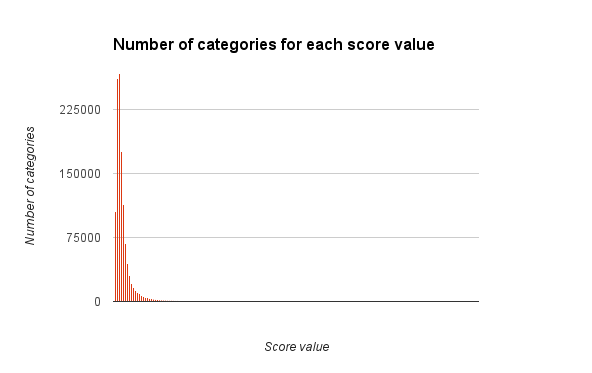
\includegraphics[width=\textwidth]{Chapters/Implementation/Grading/Inlinkoutlink_scorevalue_numberofcategories}
\caption{Number of categories for each possible score value}
\label{fig:scorevalue}
\end{figure}

%This means that the score for all categories are between 0.376010 and 6512.120784.

%This means that the scores for all categories are in the range of 0 and

%Maxgrade: 6512.120784 (albums by artist)
%Mingrade: 0.376010 (user bho-4)
\subsection{Problems with the simplified grader}
Since it is desirable with the lowest score as possible, the first problem encountered was that the program favoured short paths. 

\begin{figure}
\centering
\begin{lstlisting}
argentines of serb descent:
* society/ethnicity/ethnicity stubs/ (34.592939)
* culture/ethnicity/ethnicity stubs/ (29.704807)
* humans/ethnic groups/ethnology/ethnicity stubs/ (27.824755)
\end{lstlisting}
\caption{Caption}
\label{fig:my_label}
\end{figure}

This is both correct and wrong at the same time. It is desirable to find short paths, but there should be some punishment if the path is too short?

\begin{comment}
Problem med Alexander Huges: han er fotballspiller og dette kommer ikke så godt fra. 

asd.,kas.kdfj
\end{comment}


\begin{figure}[h]
\centering
\begin{lstlisting}
alexander hughes:
*health/health by city/health in edinburgh/sport in edinburgh/sports teams in edinburgh/football clubs in edinburgh/heart of midlothian f.c./heart of midlothian f.c. players (37.22501)
*nature/life/births by year/year of birth missing (28.576777)
*people/people categories by parameter/people by time/births by year/year of birth missing (28.200766)
\end{lstlisting}

\caption{Caption}
\label{fig:alexanderhughes}
\end{figure}
